\section{Aufbau und Durchf"uhrung}
	\label{sec:durchfuehrung}
	F"ur diesen Versuch durchl"auft das R"ontgenlicht eine Blende, wodurch ein Strahl erzeugt wird.
	Dieser trifft auf einen Drehbaren Kristall mit Gitternetzabstand $d = \SI{201}{\pico \meter}$.
	Hier wird der Strahl unter Braggbedingungen reflektiert, wobei lediglich die In\-ter\-fe\-renz\-ord\-nung $n = 1$ auftritt.
	Der reflektierte und gebeugte Strahl wird schlie"slich von einem Im\-puls\-ra\-te\-me\-ter detektiert.
	An diesem lassen sich zus"atzlich die zu untersuchenden Materialien befestigen.
	
	\begin{figure}[h]
		\centering
		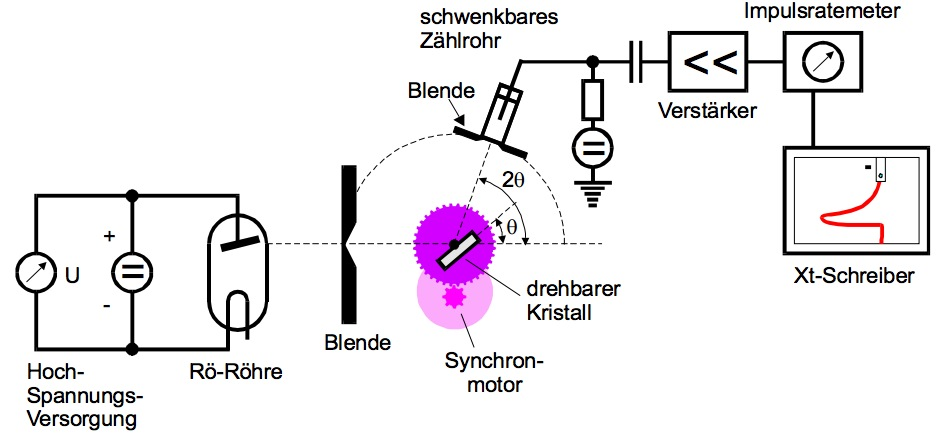
\includegraphics[width = 15cm]{img/aufbau.JPG}
		\caption{Versuchsaufbau \cite{anleitung}}
		\label{fig:aufbau}
	\end{figure}
	
	Das so gewonnene Signal kann nun am PC als Intensit"at $I$ gegen den Winkel $\theta$ aufgetragen werden.
	Es ist zu beachten, dass dieses Signal lediglich eine Mittelung "uber etliche R"ontgenquanten ist.
	Pl"otzliche Impuls"anderungen, die z.B. an den Absorptionskanten auftreten werden somit nicht scharf aufgel"ost.

	Alle Messungen wurden vollautomatisch durchgef"uhrt.
	Nachdem die zu untersuchende Probe vor dem Z"ahlrohr eingespannt wurde, konnte die Winkelaufl"osung und der Win\-kel\-be\-reich eingestellt werden.
	Die Messapparatur lieferte dann ein Signal, welches direkt am PC visualisiert und gespeichert wurde.
	Hierf"ur wurde die Software "`measure 4.6.10"' vom Apparaturhersteller PHYWE genutzt.

	\subsection{Messaufgaben}
		\begin{enumerate}
			\item{Abschirmzahl $\sigma_{1,0}$ von ${}_{32} \mathrm{Ge}$ und ${}_{41} \mathrm{Nb}$ aus den K Absorptionskanten.}
			\label{aufg:1}
			\item{Abschirmzahl $s_{2,1}$ von ${}_{79} \mathrm{Au}$ und ${}_{80} \mathrm{Hg}$ aus den $\mathrm{L}_\mathrm{II}$ und $\mathrm{L}_\mathrm{II}$ Absorptionskanten.}
			\label{aufg:2}
			\item{Sch"atzung der Abschirmzahlen $\sigma_{1}$ und $\sigma_{2}$ f"ur ${}_{28} \mathrm{Cu}$ ohne Ber"ucksichtigung des Drehimpulsbeitrages aus den Emissionsenergien $\mathrm{L}_\mathrm{K_\mathrm{\alpha}}$ und $\mathrm{L}_\mathrm{K_\mathrm{\beta}}$.}
			\label{aufg:3}
			\item{Das energetischen Aufl"osungsverm"ogen der Apparatur.}
			\label{aufg:4}
		\end{enumerate}

